\documentclass[runningheads]{llncs}
\usepackage[T1]{fontenc}
\usepackage{booktabs}
\usepackage{graphicx}
\usepackage{array}
\setlength{\emergencystretch}{2em}

\begin{document}
\title{Supplementary Material: Adaptive Test-Time Compute for Small Reasoning Models}
\titlerunning{Supplementary Material: Adaptive Test-Time Compute}
\author{Dinh-Hong Vu \and The-Tai Phung \and Thai-Son Bui}
\authorrunning{Dinh-Hong Vu, The-Tai Phung and Thai-Son Bui}
\institute{Faculty of Information Technology, Ton Duc Thang University, Ho Chi Minh City, Vietnam}
\maketitle

\section{S1. Historical Qwen3-1.7B Characterization}

These figures report the historical GSM8K grid on 99 included problems and
one stochastic generation seed. They motivate the later staged policy design
but are not pooled with the primary Qwen3-0.6B results.

\begin{figure}[!ht]
\centering
\begin{minipage}[t]{0.49\textwidth}
\centering
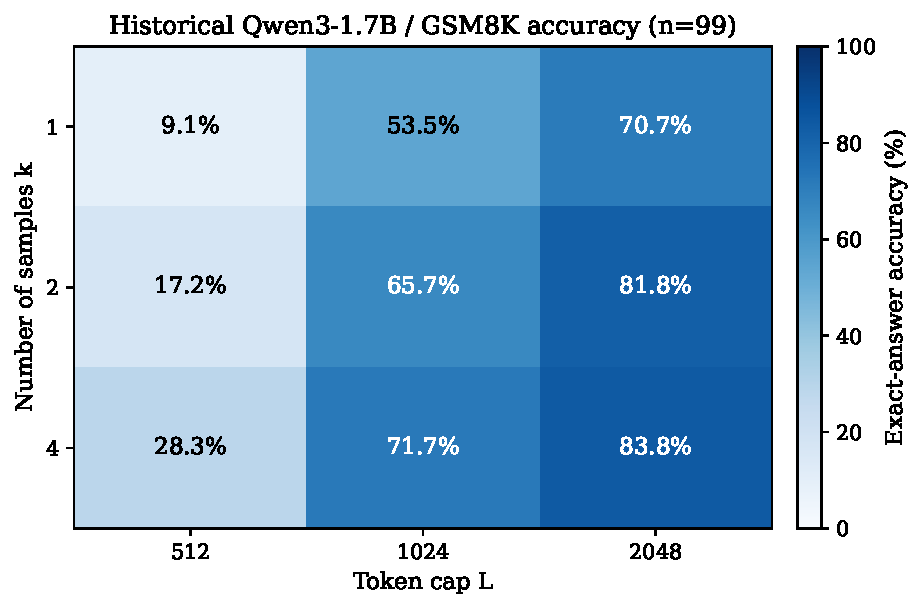
\includegraphics[width=\linewidth]{figures/historical_accuracy_heatmap_round3.pdf}
\caption{Exact-answer accuracy over the historical grid.}
\end{minipage}\hfill
\begin{minipage}[t]{0.49\textwidth}
\centering
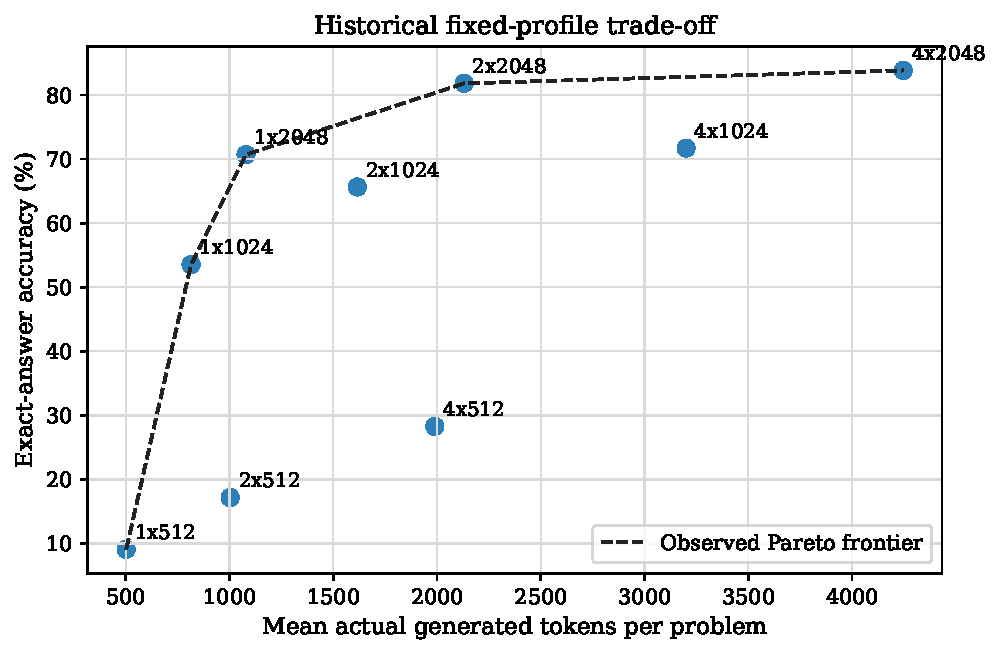
\includegraphics[width=\linewidth]{figures/historical_fixed_pareto_round3.pdf}
\caption{Observed fixed-profile accuracy--token trade-off.}
\end{minipage}
\end{figure}

\begin{table}[!ht]
\caption{Historical accuracy with Wilson 95\% intervals ($n=99$).}
\centering
\small
\begin{tabular}{ccrc@{\hspace{8mm}}ccrc}
\toprule
$k$ & $L$ & Accuracy & Wilson 95\% CI & $k$ & $L$ & Accuracy & Wilson 95\% CI \\
\midrule
1 & 512  & 9.1\%  & [4.9, 16.4] & 2 & 1024 & 65.7\% & [55.9, 74.3] \\
1 & 1024 & 53.5\% & [43.8, 63.0] & 2 & 2048 & 81.8\% & [73.1, 88.2] \\
1 & 2048 & 70.7\% & [61.1, 78.8] & 4 & 512  & 28.3\% & [20.4, 37.8] \\
2 & 512  & 17.2\% & [11.0, 25.8] & 4 & 1024 & 71.7\% & [62.2, 79.6] \\
  &      &         &              & 4 & 2048 & 83.8\% & [75.3, 89.8] \\
\bottomrule
\end{tabular}
\end{table}

\section{S2. Historical Paired Diagnostics}

Table S2 reports exact paired McNemar diagnostics. Holm correction is applied
separately to adjacent-depth, adjacent-breadth, and equal-budget families.
Zero shorter-only counts are observed in all six depth comparisons, but only
the $k=1$ monotonicity follows from the decoding and parsing contract.

\begin{table}[!ht]
\caption{Historical paired diagnostics ($n=99$). A/B are discordant counts.}
\centering
\footnotesize
\begin{tabular}{llrrrrc}
\toprule
Family & $A\rightarrow B$ & A-only & B-only & Exact $p$ & Holm $p$ & Result \\
\midrule
Depth & $1{\times}512\rightarrow1{\times}1024$ & 0 & 44 & 1.14e-13 & 5.68e-13 & sig. \\
Depth & $1{\times}1024\rightarrow1{\times}2048$ & 0 & 17 & 1.53e-5 & 4.58e-5 & sig. \\
Depth & $2{\times}512\rightarrow2{\times}1024$ & 0 & 48 & 7.11e-15 & 4.26e-14 & sig. \\
Depth & $2{\times}1024\rightarrow2{\times}2048$ & 0 & 16 & 3.05e-5 & 6.10e-5 & sig. \\
Depth & $4{\times}512\rightarrow4{\times}1024$ & 0 & 43 & 2.27e-13 & 9.09e-13 & sig. \\
Depth & $4{\times}1024\rightarrow4{\times}2048$ & 0 & 12 & 4.88e-4 & 4.88e-4 & sig. \\
\midrule
Breadth & $1{\times}512\rightarrow2{\times}512$ & 0 & 8 & 0.0078 & 0.0234 & sig. \\
Breadth & $2{\times}512\rightarrow4{\times}512$ & 0 & 11 & 0.0010 & 0.0049 & sig. \\
Breadth & $1{\times}1024\rightarrow2{\times}1024$ & 0 & 12 & 0.0005 & 0.0029 & sig. \\
Breadth & $2{\times}1024\rightarrow4{\times}1024$ & 0 & 6 & 0.0313 & 0.0625 & inc. \\
Breadth & $1{\times}2048\rightarrow2{\times}2048$ & 0 & 11 & 0.0010 & 0.0049 & sig. \\
Breadth & $2{\times}2048\rightarrow4{\times}2048$ & 0 & 2 & 0.5000 & 0.5000 & inc. \\
\midrule
Equal budget & $4{\times}512\rightarrow2{\times}1024$ & 1 & 38 & 1.46e-10 & 3.94e-10 & sig. \\
Equal budget & $4{\times}512\rightarrow1{\times}2048$ & 3 & 45 & 1.31e-10 & 3.94e-10 & sig. \\
Equal budget & $2{\times}1024\rightarrow1{\times}2048$ & 8 & 13 & 0.3833 & 0.3833 & inc. \\
\bottomrule
\end{tabular}
\end{table}

\clearpage
\section{S3. Non-Thinking Validation Control}

This post-primary control uses the same frozen Validation-20 problems, model
revision, prompts, sampling settings, and high cap. It did not access or alter
Test-100.

\begin{table}[!ht]
\centering
\caption{Paired thinking versus non-thinking results. Each cell gives correct
problems and mean actual generated tokens.}
\small
\begin{tabular}{llr@{\hspace{8pt}}r@{\hspace{8pt}}r}
\toprule
Data & $(k,L)$ & Thinking & Non-thinking & Token saving \\
\midrule
GSM8K & $(1,2048)$ & 13/20; 986.15 & 1/20; 31.30 & 96.83\% \\
GSM8K & $(2,2048)$ & 14/20; 1,969.70 & 1/20; 84.85 & 95.69\% \\
GSM8K & $(4,2048)$ & 15/20; 3,593.85 & 1/20; 143.65 & 96.00\% \\
MATH & $(1,4096)$ & 11/20; 2,388.70 & 8/20; 471.90 & 80.24\% \\
MATH & $(2,4096)$ & 13/20; 4,700.50 & 8/20; 923.40 & 80.36\% \\
MATH & $(4,4096)$ & 13/20; 8,979.10 & 11/20; 1,972.50 & 78.03\% \\
\bottomrule
\end{tabular}
\end{table}

\section{S4. Complete Agreement-Stopping Measurements}

\begin{table}[!ht]
\centering
\caption{Held-out two-sample stopping results. Saving is relative to fixed
$k=4$ at the same cap. Prediction equality was verified for every row.}
\small
\begin{tabular}{l@{\hspace{7pt}}r@{\hspace{7pt}}r@{\hspace{7pt}}r@{\hspace{7pt}}r@{\hspace{7pt}}r@{\hspace{7pt}}r}
\toprule
Data & $L$ & Stop at 2 & Continue to 4 & Mean tokens & Saving & Accuracy \\
\midrule
GSM8K & 512  & 28 & 72 & 1,601.83 & 11.57\% & 53/100 \\
GSM8K & 1024 & 54 & 46 & 1,994.52 & 21.33\% & 76/100 \\
GSM8K & 2048 & 62 & 38 & 2,455.01 & 24.25\% & 76/100 \\
MATH-500 & 1024 & 11 & 89 & 3,776.01 & 4.01\% & 17/100 \\
MATH-500 & 2048 & 37 & 63 & 5,894.19 & 12.97\% & 50/100 \\
MATH-500 & 4096 & 57 & 43 & 8,191.12 & 19.96\% & 73/100 \\
\bottomrule
\end{tabular}
\end{table}

\end{document}
